\documentclass[
	msc,
	english
%% Para dissertações de mestrado, OU
%	mscproposta, %% Para propostas de dissertação de mestrado, OU
%	phd, %% Para teses de doutorado, OU
%	phdproposta, %% Para propostas de tese de doutorado
%	portugues %% Para documentos em português, OU
%	english %% Para documentos em inglês
]{ppgccufmg}

%\usepackage[brazil]{babel} %% se o documento for em português, OU
\usepackage[english]{babel} %% se o documento for em inglês
%\usepackage[latin1]{inputenc}
\usepackage{natbib}
\usepackage{xcolor}
\usepackage{lipsum}
\usepackage[
	colorlinks=true,
	linkcolor=blue, %% Cor dos links do sumário
	citecolor=red, %% Cor dos links das citações      
	urlcolor=magenta, %% Cor das urls
]{hyperref}
\usepackage{amsmath}
\usepackage{amssymb}
\usepackage{minted}
\usepackage{algorithm}
\usepackage{algpseudocode}
\usepackage[toc]{glossaries}
\usepackage{glossaries-extra}
\usepackage{bm}
\usepackage{tikz}
\usepackage{relsize}
\usepackage[normalem]{ulem}
\usepackage{stmaryrd}
\usepackage{proof}
\usepackage{mathtools}
\usepackage{amsfonts}
\usepackage{amsthm}
% \usepackage[proofrulebaseline=2ex]{prooftrees}


%% Exemplo de lista customizada ==================
%% Para criar uma lista customizada (como Lista de Algoritmos, Lista de Exemplos) que ficará juntamente com as Lista de Figuras e Lista de Tabelas, execute os 3 comandos abaixo substituindo "algoritmos" pelo tipo de lista que estará criando. Para adicionar a lista ao documento, deverá passar o seguinte parâmetro no comando \ppgccufmg:
%% \ppgccufmg{
%% 		...
%% 		listacustomizada={\listadealgoritmos}
%% }
% \newfloat[chapter]{algoritmo}{lol}{Algoritmo}
% \newcommand{\listaalgoritmosname}{Lista de Algoritmos} %% Título da lista
% \newlistof{listadealgoritmos}{lol}{\listaalgoritmosname} %% O primeiro parâmetro é o nome da lista, e este deverá ser passado no parâmetro listacustomizada={\nomedalista}
% \newlistentry{algoritmo}{lol}{0} %% Nome do ambiente de cada algoritmo, e.g., \begin{algoritmo} ... \end{algoritmo}

%% **** Caso não haja nenhuma lista adicional, os comandos acima podem ser apagados. ****
%% ===============================================

\DeclareUnicodeCharacter{2200}{$\mathbb{\forall}$}

\newtheorem{theorem}{Theorem}
\newtheorem{definition}{Definition}
\newtheorem{example}{Example}

\newcommand{\yell}[1]{{\color{blue} [#1]}}
\newcommand{\tom}[1]{\yell{#1 --tom}}

\newglossarystyle{mystyle}{%
  \glossarystyle{long}%
  \renewenvironment{theglossary}%
     {\begin{longtable}{p{3cm}p{\glsdescwidth}}}%
     {\end{longtable}}%
}

\newglossary{symbols}{sym}{sbl}{List of Symbols}
\makeglossaries
% \newglossaryentry{NegLit}
% {
%     name = {$\bm{\overline x}$ },
%     description={Negation of the literal $x$}
% }
\newglossaryentry{IncVar}
{
  name = {$\bm{x \in C}$ },
  description={Variable $x$ is present in the clause $C$}
}
\newglossaryentry{RemVar}
{
  name = {$\bm{C \setminus x}$ },
  description={Clause $C$ without variable $x$}
}
\newglossaryentry{FormulaVars}
{
  name = {$\bm{\textit{Vars}(\psi)}$ },
  description={Set of all variables in the formula $\psi$}
}
\newglossaryentry{Resolution}
{
  name = {\bm{$C_{1} \diamond_{x} C_{2}$} },
  description={Clause resulting from applying resolution with $C_{1}$ and $C_{2}$ using $x$ as a pivot}
}
\newglossaryentry{VarAssign}
{
  name = {$\bm{\psi_{\{x \gets val\}}$} },
  description = {Formula resulting of assigning the variable $x$ to the boolean value $val$ in $\psi$}
}

\begin{document}
	\ppgccufmg{
		autor={Tomaz Mascarenhas}, %% Autor(a)
		titulopt={Demonstrando teoremas em Lean por meio da reconstrução de demonstra\c{c}\~oes em SMT},
		tituloen={Proving Lean theorems via reconstructed SMT proofs}, %% Título em inglês
		cidade={Belo Horizonte},
		ano={2023},
		versaopt={Final},
		versaoen={Final}, %% Palavra que acompanhará 'Version' na folha de rosto em inglẽs
		orientador={Haniel Barbosa}, %% Para masculino
		% fichacatalografica={fichacatalografica.pdf},
		% folhadeaprovacao={folhadeaprovacao.pdf},
		resumo={resumo.tex}, %% Resumo em português
		palavraschave={Verifica\c{c}\~ao Formal, Lean, SMT},
		abstracten={abstract.tex}, %% Abstract em inglês
		keywords={Formal Verification, Lean, SMT}, %% Palavras-chave do abstract
		% dedicatoria={dedicatoria.tex}, %% Arquivo .tex contendo a dedicatória
		% agradecimentos={agradecimentos.tex},
		epigrafe={S\'o quem sonha acordado v\^e o sol nascer.},
		epigrafeautor={Unknown},
		% listadefiguras={sim}, %% Remova (ou comente) este parâmetro para remover a lista de figuras
		% listadetabelas={sim}, %% Remova (ou comente) este parâmetro para remover a lista de tabelas
		% listascustomizadas={\listadealgoritmos} %% Lista customizada (e.g., lista de algoritmos).
	}

    \printunsrtglossary %[style=mystyle]

	\newpage

	\tableofcontents

	\chapter{Introduction}
	  \section{Context}
	    A mechanized proof is a proof, written in some language recognized by a computer, that had its validity checked by a trusted verifier. One of the main applications of these artifacts are formalizing mathematical theories. Indeed, there are well-known examples of successful formalizations. One of them is the mechanization of the proof of a theorem regarding Perfectoid Spaces\cite{scholze}, done by the fields-medalist mathematician Peter Scholze, together with the community of a system called Lean\cite{lean}. Scholze proved the theorem using pen and paper, but was unsure of the result due to its complexity. Once he translated the theorem and the proof to the language of Lean, the system could point out some mistakes he made, and, after fixing them, he could be sure of the correctness of the proof.

Another application of mechanized proofs is verifying the correctness of mission-critical software. Given a specification of the behavior of some program, the program is said to be correct if it respects the specification for any input it is given. For instance, one could specify that a sorting routine must always produce the sorted permutation of it's input list. In this case, a given sorting routine is said to be correct if it indeed produces the desired permutation, regardless of which list it receives. There are a variety of techniques to obtain correctness evidence for a software. The most common one is the development of tests. Besides being easy to write an efficient set of tests, there are many types of bugs that can be discovered with its execution. In fact, this approach is enough for a large amount of problems that are solved by software engineering. However, tests can’t guarantee that a program doesn’t have flaws, since the number of valid inputs is almost always exceedingly large, or infinite. This kind of guarantee is extremely important for mission-critical software, that is, systems that have critical responsibilities, such as the control of airplanes or medical equipment. In this context, one promising alternative is to use a mechanized proof of the correctness of the software as an evidence for its safety.

The process of generating mechanized proofs can be divided into
two categories: interactive and automatic.

Interactive theorem provers (ITPs) are mainly represented by proof assistants, in which, after defining
a theorem, the user attempts to manually write a proof for it,
relying on the tool to organize the set of hypothesis and
how the goal changed step-wisely through the proof, as well as to ensure the
correctness of each step according to a trusted kernel.
%
In order to keep the kernel simple and small (and, therefore, easy to be trusted), it's implementation usually just straightforwardly checks the logic rules from the logic implemented by the ITP.\ Because of this, each step must be explicitly stated by the user, making the tool costly to be used.
% %
% Each logic step must be explicitly stated by the user, which makes the tool
% costly to be used.

Automatic theorem provers (ATPs), on the other hand,
only require the user to define a conjecture, proceeding automatically to
determine whether there exists a proof for it, or possibly providing a
counter-example if it can find one.
%
Although they are easier to use, ATPs require a large
codebase to implement all the algorithms necessary to execute the search for a proof,
making them more susceptible to errors and harder to be trusted.
One possible way to overcome this trust issue is to produce
a mechanized proof verifying the correctness of the ATP, however,
besides being a very complex task, once the proof is done the
development of the ATP becomes freezed, otherwise it would
have to be verified again.

Another approach to increase the confidence in ATPs is to have them provide a
proof to support their results, so that it can be independently verified whether
it indeed proves the theorem in question. This has the downside of creating a need
for allocating resources to verify the proof of every single theorem that is proved.
On the other hand, as long as the proof format doesn't change, the implementation
of the solver can be modified without requiring a modification in the checkers. Also,
it is important to consider that it is often simpler to verify proofs than to verify
the tool itself.

Another important advantage of the second approach is that it allows the ITPs to leverage the automatic proving performed by the ATPs by using the proofs they produce, since the requirement for accepting a proof, i.e.\ that each step is correct to its internal logic,
can be applied to the ATP proof.
%
By connecting these systems, it would be possible for the user of the ITP to focus on more complex steps of the proof, such as defining an induction hypothesis, while delegating the burden of other long and straightforward steps to the ATP.\ Indeed, this
connection is so important that there are projects like Hammering Towards QED~\cite{hammering}
that outline all the efforts that were already made in order to integrate
interactive and automatic theorem provers. In this paper, the authors describe in detail each component that a system that creates a connection between ATPs and ITPs has to implement, as well as the main issues that they have to solve, based on existing programs that were successful in this task. Besides that, they show their potential through several large benchmarks. 


	  \section{Contributions}
	    Given this context, we present a set of tools that would be an essential
part of the integration between the ITP Lean 4~\cite{lean} and the SMT solver cvc5~\cite{cvc5}.
%
Specifically, we aim to build a system that takes proofs of the unsatisfiability of
SMT queries produced by cvc5 and reconstructs them in Lean.
%
The main motivation of this project is that despite the fact that Lean is
emerging as a promising programming language and proof assistant and being
widely used by mathematicians in large-scale
formalizations~\cite{mathlib, scholze}, there is currently no way to
interact with SMT solvers from it, even though these systems have been
central in previous developments of proof automation in ITPs, as we will show in Sections~\ref{sec:smtcoq}
and~\ref{sec:sledgehammer}. The contribution of the present work
would enable a faster development of this kind of project using Lean.

We use the cvc5 solver because it already has a module for exporting proofs as
Lean scripts~\cite{Barbosa2022}, using a representation of the SMT terms\footnote{For more details
about the SMT term language, see SMT-LIB~\cite{smtlib}.} as an inductive type in Lean.
However, these proofs are not fully verified by Lean's checker. Instead, a set of
axioms are declared in Lean, representing all the logical rules that cvc5 uses to prove
theorems, and the ITP only checks whether the rules were applied correctly and whether
the end result of applying all the rules in the proof is, indeed, the required one.
Our main contributions are to eliminate the need of increasing the trusted base by introducing
those axioms and to make the proofs operate over native Lean terms, as opposed to terms
of the inductive type that represents SMT terms.

Note that the set of tools we are proposing does not implement the full integration
between Lean and cvc5. For instance, we do not implement a module for translating
Lean goals into an equivalent SMT problem. However, our project is being used
as part of the joint project Lean-SMT\footnote{The code for the project can be found at \url{https://github.com/ufmg-smite/lean-smt}}, that aims to implement a tactic in Lean
that would perform the complete process, that is, starting from a Lean goal, translating it to a SMT query, invoking a solver to try to prove it and lifting the proof produced (in case it is found) to Lean's language, so that it can be used as a proof for the original goal.

	  \section{Related Work}
	    \subsection{Hammering Towards QED}
           \label{sec:hammering}
			\label{sec:hammering}
As previously mentioned, Hammering Towards QED is a project
that aims to describe all the tools, which the paper calls ``hammers'',
that were created with the purpose of connecting automatic and interactive
theorem provers. Besides that, this document also outlines
the main components that such tools usually have. They are
the following:

\begin{itemize}
  \item The premiss selection module: that identifies
        a subset of the facts previously demonstrated in the
        ITP that are more likely to be useful in order to
        prove the given goal, to be dispatched to the ATP.\@
  \item The translation module: that builds a problem in the language of the
        ATP that corresponds to the original goal from the ITP and using
        the premisses that were selected.\@
  \item The proof reconstruction module: that lifts the proof produced
        by the ATP into a proof that is accepted by the ITP.\@
\end{itemize}

In our case, we will restrict ourselves to implement a proof reconstruction module.
The three main strategies used to reconstruct the proof produced
by the automatic system inside the interactive one are also described in the paper.

The first one is to use the ITP to verify a deeply embedded version of the proof
received, and, in case it is succesful, reflect this proof inside it's checker, proving
the original goal. More specifically, the hammer defines a datatype to represent
terms in the ATP and a set of functions to manipulate values on those datatypes, representing
the axioms that the solver uses to transform the terms. Then, a lifting function is defined, that is,
a function that take a value of this datatype and outputs an equivalent term in the native
language of the ITP.\ Finally, the correctness of each transformation function is
verified with respect to the lifting function, in the sense that, if the input term
was lifted to a value that is provable in the ITP's logic, then the output term will
also be provable. The ATP's proof will be represented as a sequence of those
transformations, and their correctness are proved \textit{a priori}. When checking
a specific proof, the only step that the ITP must perform is to compute the result
of the application of all the functions in the solver's output, and to check if
the final term matches with the expected one. This technique is known as
the Certified approach\ \cite{snipe}.

The second one is to match each axiom in the ATP's logic into a proved lemma or a tactic
\tom{is it okay to use tactic here? should I introduce the term first?}
defined in the ITP that works directly with native terms of the system.
The proof produced by the automatic solver is then parsed into a sequence of applications
of those lemmas and tactics and replayed inside the ITP.\ In this case, the proof is built
on the fly and does not have it's correctness guaranteed (it can fail in the middle of the
proccess in case the ATP or the hammer did something wrong). On the other hand,
this technique skips computations done over embedded terms, which have to be done by the
Certified approach, having the potential to have a better
performance. This approach is known as the Certifying approach\ \cite{snipe}.

The third one is to compile the proof into the ITP's source code. This implies generating
an actual script in the native language of the interactive system
that corresponds to the proof received. After the script is generated, it is
possible to postprocess\tom{maybe copy the references that hammering towards use to talk about this?}
it in order to make the proof easier to be checked,
in a way that the final script can possibly ignore a large portion of the
original proof. This approach can be inconvenient for very large proofs,
as it requires that the script is stored in some filesystem. However,
it has the advantage over the two previous methods of only requiring access to the ATP
on the first time that the proof is checked.

In this project we will be using the second approach. We give more details about this
decision in the later chapters.

	    \subsection{SMTCoq}
           \label{sec:smtcoq}
			One notable example of such integrations is SMTCoq~\cite{smtcoq}.
It is a plugin for the proof assistant Coq~\cite{Bertot2004} that
can be used as a tactic to prove theorems via their encoding into
SMT and by lifting proofs produced by the SMT solvers veriT~\cite{Bouton2009}
and CVC4~\cite{Barrett2011}. The tool relies on a preprocessor written in OCaml
to transform proof witnesses coming from different solvers into certificates in
the Coq language. The system has a set of checkers for each theory in SMT, each
one of them consisting of theorems asserting the validity of certain transformations
in the SMT terms. All those checkers are connected by the main checker, that
is essentially a theorem stating that if all the transformations resulted in an
empty clause, then the lifting of the original term is false, for any instantiation
of its free variables. This kind of reasoning is known as proof by computational
reflection~\cite{reflection} which is an instance of Certified Transformations, which will be described
in Section~\ref{sec:certifiedVsCertifying}.

		\subsection{Sledgehammer}
           \label{sec:sledgehammer}
			The ITP Isabelle/HOL~\cite{Nipkow2002} has a similar tool,
namely, Sledgehammer~\cite{sledgehammer}. This system achieves its goal by
invoking several SMT solvers in parallel to prove a given goal and collecting
their output to determine which lemmas must be applied in order to prove the theorem
inside Isabelle. In a way, this approach is very similar to the one we're using in this project, as the proof is produced on
the fly (known as the Certifying approach, which will also be described in Section~\ref{sec:certifiedVsCertifying}) as opposed
to having a single theorem that establishes once and for all
that, if all steps performed by the solver were successful,
then the original goal is valid, as is done by SMTCoq.

	  \section{Organization of this document}
	    In Chapter~\ref{chap:formalPrelim} we present the concepts involved in our work.
We describe the SMT problem in detail, as well as the main techniques used to solve
it and the proof certificates produced by cvc5. We also present Lean and give
an overview of the features of the language we have employed throughout the project.
%
Then, in Chapter~\ref{chap:certified}, we describe the steps necessary to implement
the reconstruction of proofs from cvc5 in Lean using the approach of certified
transformations.
%
Next, in Chapter~\ref{chap:rcons}, we present in detail our implementation of the
reconstruction using the certifying transformations approach.
%
This implementation is evaluated in Chapter~\ref{chap:eval}.
%
Finally, we present some possible directions for future work in
Chapter~\ref{chap:future}.

	\chapter{Formal Preliminaries}
	  \section{Satisfiability Modulo Theories (SMT)}\label{sec:smt}
	    \subsection{Description of the Problem}

The Boolean Satisfiability Problem (SAT) consists of, given a formula in Propositional Logic (PL) containing free variables, determine whether exists a function that assigns each variable to a boolean value, in a way that, after replacing the variables by their values provided by the function, the formula is evaluated to \textit{true}. We say that a formula is satisfiable if such function exists, and unsatisfiable otherwise. In this work, we will be focusing on the problem CNF-SAT, an equivalent version of SAT in which the input formula always comes in Conjuctive Normal Form, that is, a conjunction of disjunctions. From now on, we will use SAT to refer to the CNF-SAT problem. Besides that, we will use the name \textit{clause} to refer to one of the disjunctions in some input formula for SAT.

Satisfiability Modulo Theories (SMT)~\cite{smt} is a generalization of SAT.\ There are two additions in this version of the problem: the first one is that the input formula can contain quantifiers binding variables, which will affect the satisfiability of that formula. Therefore, any formula in First Order Logic is a valid input to the SMT problem. The second addition is the inclusion of a set of theories that allows the problem to refer to variables of different domains. More precisely, a theory consists of a sort (for instance, integers) over which a subset of the variables of the problem can range over and a set of symbols that represents operations over these sorts with predefined semantics (for instance, addition and comparison operations). Note that SMT problems are allowed to use multiple theories in the same instance. The logic framework that corresponds to Propositional Logic with these two additions is known as Many-Sorted First Order Logic (MSFOL). The semantics of this logic is given in detail in~\cite{many_sorted}. In the next section we give a brief overview of it.

% EXAMPLE -- remove?

% For instance, let $x$ and $y$ be integer variables and the symbols $+$ and $<$ have their usual meaning of addition and comparison of integers. Then, consider the formula:

% \begin{center}
%   $0 < x \land x < 2 \land (\forall z . (y < z) \lor x + y < 1 + y)$
% \end{center}

% By the first two propositions we can derive that $x = 1$. But if $x = 1$ then $x + y$ can't be lesser than $1 + y$. Also, it is impossible to choose a value for $y$ such that $\forall z . (y < z)$. Therefore, there is no value for $x$ and $y$ that would satisfy the whole formula. In other words, it is unsatisfiable. On the other hand, the following formula is satisfied by assigning, for instance, $x = 0$ and $y = 3$:

% \begin{center}
%   $-1 < x \land x < 1 \land (\forall z . (y < z) \lor x + y < 1 + y)$
% \end{center}

% END EXAMPLE

% tem que falar o que eh uma demonstracao nesse contexto antes de falar isso
% Some of the most relevant theories in SMT are Linear Integer Arithmetic (LIA), Linear Real Arithmetic (LRA), Bitvectors (BV) and Equality and Uninterpreted Functions (EUF).
% In this work, we will focus on reconstructing proofs from LIA, LRA, EUF and regular SAT proofs of unsatisfiability.

\subsection{Applications}

Given a program and a formal specification of some property related to the program, it is often \tom{always?} the case that we can express the proposition that asserts that the program satisfy the property as an SMT instance. For instance, consider the well known \textit{abs} function, that takes an integer and returns its absolute value. The usual way to implement it is through a branch that checks whether the input variable is positive or negative. In case it is positive, its own value is returned. Otherwise, the value multiplied by $-1$ is returned:

\begin{algorithm}
\caption{Original Absolute Function}~\label{originalAbs}
\begin{algorithmic}
\Function{abs}{x}
\If{$x < 0$}
  \State\Return$-x$
\Else
  \State\Return$x$
\EndIf
\EndFunction
\end{algorithmic}
\end{algorithm}

In program analysis, it is quite useful to eliminate branches from programs since this action completely removes one possible path that the flow of the program can take (besides optimizing it's performance). Obviously, this operation must be done with caution to not modify the original behavior of the program. In his book~\cite{hacker_delight}, Henry Warren proposes an alternative implementation for the \textit{abs} function which doesn't have branches:

\begin{algorithm}
\caption{Branchless Absolute Function}~\label{branchlessAbs}
\begin{algorithmic}
\Function{abs'}{x}
  \State $y \gets x >> 31$
  \State \Return $(x \bigoplus y) - y$
\EndFunction
\end{algorithmic}
\end{algorithm}

Where $\bigoplus$ represents the bitwise xor operation. We can design an instance of the SMT problem that asserts that both implementations produce the same output, when given the same input. We present the instance written in SMT-LIB~\cite{smtlib}, a standardized syntax for representing SMT problems:

\begin{minted}[linenos]{smtlib2.py -x}
(set-logic QF_BV)
(declare-const x (_ BitVec 32))
(declare-const result1 (_ BitVec 32))
(assert (= result1 (ite (bvslt x #x00000000) (bvneg x) x)))
(declare-const y (_ BitVec 32))
(declare-const result2 (_ BitVec 32))
(assert (= y (bvashr x (_ bv31 32))))
(assert (= result2 (bvsub (bvxor x y) y)))
(assert (distinct result1 result2))
(check-sat)
\end{minted}

First, we set the combination of theories that will be used in this problem. In our case, we will be using \textit{QF\_BV}, which stands for quantifier free bitvectors. This means that this instance of the problem is not allowed to use quantifiers and is allowed to declare and use variables living in the Bitvector sort, as well as operations over this sort. Bitvectors are fixed-length arrays of bits. They are useful for representing machine integers, as they can simulate their semantics.

Next, in lines 2 and 3, we define two constants, both from the sort \textit{BitVec 32} (arrays of 32 bits): \textit{x} and \textit{result1}. The first one represents the input value from the original \textit{abs} function, and the second one, the result produced by that function. We then have to add an assertion in line 4 that binds the variable \textit{result1} to the output of the function \textit{abs} in terms of \textit{x}. We translate the branch from the pseudocode as the \textit{ite} operator, the comparison as the \textit{bvslt} operator and the multiplication by -1 as the \textit{bvneg} operation. This assertion will be encoded as a regular implication from SAT, where the premiss is it's proposition and the conclusion is the rest of the problem, which still needs to be defined. In lines 5 to 8 we repeat the process to define \textit{y} and \textit{result2}, which corresponds to the result of the branchless \textit{abs} function. Finally, we assert that \textit{result1} and \textit{result2} must be different in line 9. If this problem is satisfiable, then there is a value for \textit{x} which produces different values in each function. If it is unsatisfiable, then we can be sure that no such value exists, therefore, both functions are equivalent. Note that we are not verifying that the actual code of the functions are equivalent, just an abstraction over it's implementation.

% Given that we have very efficient systems to solve such problems, which will be introduced later, the possibility of formally verifying programs using this technology is quite promising. Indeed, \tom{pegar referencias do paper do leonardo (https://fm.csl.sri.com/SSFT14/smt-application-chapter.pdf)}
%

% \begin{itemize}
%   \item revolucao sat
%   \item representar propriedades de programas como problemas smt
%   \item geracao de casos de teste
%   \item geracao de programas
%   \item F*, Dafny
% \end{itemize}

\subsection{Many-Sorted First Order Logic}

define formarly many sorted first order logic

talk about fixing the meaning of some theories to improve performance

skipping this for now, I will write the rest of the thesis so I have a better understanding of what needs to go here

\subsection{SMT Solvers}

A SMT solver is a piece of software whose main goal is to solve the SMT problem. Many-Sorted First Order Logic is undecidable in it's most general form~\cite{fol_undec}, therefore SMT solvers have to limit themselves to use heuristics to solve the largest possible subset of instances of the problem. In this section we present the ideas used by these systems that are most relevant to the present work.

\subsubsection{DPLL}

First, let’s explore how SAT is solved. Although MSFOL is not decidable, Propositional Logic is, therefore, it is possible to design a decision procedure for SAT.\@ Indeed, one simple way to check whether a formula in PL with $n$ variables is satisfiable or not is to simply test each one of the $2^{n}$ functions assigning truth values to those variables.

A more efficient alternative of a decision procedure for PL is the DPLL algorithm~\cite{dpll}. DPLL is based on the \textit{Resolution} theorem:

\begin{theorem}[Resolution]
Let $x$ be a literal. Let $C_{1}$ and $C_{2}$ be two clauses such that $x \in C_{1}$ and $\overline x \in C_{2}$. Then $C_{1} \wedge C_{2} \rightarrow (C_{1} \setminus x) \vee (C_{2} \setminus \overline x)$.
\end{theorem}

More specifically, it is based on \textit{Unit Resolution} (UR), that is, a more specific version of Resolution in which $C_{1} = \{x\}$ or $C_{2} = \{\overline x\}$. We present it's pseudocode:

\begin{algorithm}[H]
\caption{DPLL Algorithm}~\label{dpllAlgo}
    \hspace*{\algorithmicindent} \textbf{Input:} $\psi$, a formula in CNF \\
    \hspace*{\algorithmicindent} \textbf{Output} \textit{true} or \textit{false}, depending whether $\psi$ is satisfiable
\begin{algorithmic}
\Function{DPLL}{$\psi$}
\If{$\exists C \in \psi .\, C = \{\bot\}$}
  \State~\Return~\textit{false}
\ElsIf{$\forall C \in \psi .\, \top \in C$}
  \State~\Return~\textit{true}
\Else
  \If{$\exists x \in Vars(\psi) \,$ such that $x$ is a target for UR}
    \State $\langle C_{1}, C_{2} \rangle \gets$ \Call{findClauses}{$x$} \Comment{Clauses suitable for applying UR with $x$}
    \State~\Return~DPLL($\psi \cup C_{1} \diamond C_{2}$)
  \Else
    \State~Let $x$ be an unassinged variable in $\psi$
    \State~\Return~\Call{DPLL}{$\psi_{\{x \gets \top\}}$} $\vee$ \Call{DPLL}{$\psi_{\{x \gets \bot\}}$}
  \EndIf
\EndIf
\EndFunction
\end{algorithmic}
\end{algorithm}

The algorithm works as follows: first, it checks to see if the formula can be evaluated to \textit{true} or \textit{false}. In case it can't, the procedure finds as many variables in which it can apply Unit Resolution as possible. Once there are no more possibilities, it chooses an arbitrary variable and make two recursive calls: one assigning this variable to \textit{true} and the other one to \textit{false}. Since these are the only two possibilities for that variable, the input formula is satisfiable if and only if one of the recursive calls returned \textit{true}. The algorithm uses this information to simply return the disjunction between the two return values.

\subsubsection{Congruence}


\subsection{Proofs in cvc5}

	  \section{Lean}
      \tom{disclaimer: for now I will just give a minimal definition on Lean's features. Later, if I discover that I need something else in the next chapter I add it here}

Lean is both an Interactive Theorem Prover and a programming
language. It is based on the Calculus of Inductive Constructions (CIC)~\cite{cic_ref} and explores the well-known correspondence between types and propositions~\cite{ch_correspondence} to implement a system that is both a proof checker and a type checker. This way, the ITP has a kernel with less than 7500 lines\footnote{Information obtained in 25/07/2023} that is powerful enough to recognize a language capable of expressing the theory of dependent types~\cite{dep_type_theory}.

\subsection{Lean as a Programming Language}

Lean has all the main features one can expect from a functional programming language. Its features include algebraic datatypes, pattern matching, polymorphism, typeclasses, IO support using monads and a robust macro system. The following script is a valid Lean program, that defines a new type representing natural numbers, together with a function for adding them:

\begin{minted}{lean}
inductive Natural where
  | zero : Natural
  | succ : Natural -> Natural

open Natural

def add (n m : Natural) : Natural :=
  match n with
  | zero    => m
  | succ n' => succ (add n' m)

notation x " + " y => add x y
\end{minted}

The keyword \textit{inductive} is used to introduce a new type, which in this case will be named \textit{Natural}. After the name, the user must use the keyword \textit{where}, followed by its constructors and their types. The constructors for the type Natural are \textit{zero} (which does not take any parameter and returns a Natural) and \textit{succ} (which takes a Natural and returns another one). This declaration introduces the constructors in the context with the names \textit{Natural.zero} and \textit{Natural.succ}. In order to be able to write just ``zero'' and ``succ'' we use the command \textit{open Natural}.

The next three lines define the sum function. We define new functions using the keyword \textit{def} followed by its name, the list of parameters and their types, the return type and the body of the function after the symbol ``:=''. In this case, we define the function by pattern matching on the first parameter. If it is \textit{zero}, we just return the second parameter. If it is \textit{succ} of some other value \textit{n'}, we return the \textit{succ} constructor applied to the result of a recursive call of \textit{add}, using \textit{n'} and \textit{m}.

Lastly, we use the command \textit{notation} to define a macro for using the add function with the usual infix ``+'' operator.

% Another useful feature of Lean is the possibility of asking for a type of a given expression. We do this with the command \textit{\#check}, followed by the expression we want to consult the type:

% \begin{minted}{lean}
%   #check add -- Natural -> Natural -> Natural
%   #check Natural -- Type
% \end{minted}

\subsection{Lean as a Theorem Prover}

In Lean, propositions are represented by types, which are inhabited by terms that represent proofs of those propositions. For instance, the following Lean expression represents a proposition (which is also a type) stating that, according to our previous definition of natural numbers, the addition of any natural \textit{n} and \textit{zero} results in \textit{n}:

\begin{minted}{lean}
∀ (n : Natural), (n + zero) = n
\end{minted}

The representation of this predicate as a type is possible due to the fact that Lean supports dependent types, that is, types that depend on values of other types. The operator \textit{=} in this expression is a type constructor that accepts two values of the same type.

Therefore, proving that this statement holds amounts to finding a term with this type. The following snippet shows the construction of such term:

\begin{minted}{lean}
theorem add_zero : ∀ (n : Natural), (n + zero) = n :=
  fun n =>
    match n with
    | zero    => rfl
    | succ n' => congrArg succ (add_zero n')
\end{minted}

This structure follows the same pattern as the one for defining functions, the only difference is the change of the keyword \textit{def} to \textit{theorem}. After the symbol ``:='' we have essentially a constructive proof of the statement. First, it introduces the variable binded by the $\forall$ symbol in the context, using \textit{fun n}. Then, it uses pattern match on \textit{n}. If \textit{n} is \textit{zero}, the type that is required is reduced to \textit{zero + zero = zero}, which follows directly from the definition of \textit{add}. The term \textit{rfl} is a proof that any term is equal to itself. In this case, Lean can match its type with the required one. If \textit{n} follows the pattern \textit{succ n'}, then the required type is \textit{succ n' + zero = succ n'}. By the definition of \textit{add}, the left-hand side evaluates to \textit{succ (n' + zero)}.
Note that the term \textit{add\_zero n'} has type \textit{n' + zero = n'}, which is almost the required one, missing only the \textit{succ} on both sides. This is solved by applying \textit{congrArg succ} on \textit{add\_zero n'} (\textit{congrArg} is a version of Theorem~\ref{cong_theorem} in Lean's library), which produces a term with the correct type.


We also present a proof that our addition function is commutative, together with another necessary lemma:

\begin{minted}{lean}
  theorem add_succ : ∀ (n m : Natural),
    (n + succ m) = succ (n + m) := fun n m =>
  match n with
  | zero    => rfl
  | succ n' => congrArg succ (add_succ n' m)

theorem add_comm : ∀ (n m : Natural), (n + m) = (m + n) := fun n m =>
  match n with
  | zero    => Eq.symm (add_zero m)
  | succ n' =>
    Eq.trans (congrArg succ (add_comm n' m)) (Eq.symm (add_succ m n'))
\end{minted}

Note that, since we have to make explicit every single logic step, even simple proofs are not easy to write and read. Lean (and most ITPs) provide an alternative for this kind of proof: the usage of tactics. As previously explained, tactics are routines that simulate common proof techniques. While we are building a proof term, Lean's kernel always keep track of a context, containing all declarations in scope and what is the currently expected type for the term we are building (also known as the goal). Tactics operate by manipulating these two structures, without compromising the trusted kernel. In other words, any modification that is made by a tactic must be properly justified and will be checked by Lean's kernel, in the same way it checked that our proof was correct.

We present a new version of \textit{add\_comm} with this new approach:

\begin{minted}{lean}
theorem add_comm' : ∀ (n m : Natural), (n + m) = (m + n) := by
  intros n m
  induction n with
  | zero       => rw [add, add_zero]
  | succ n' IH => rw [add, add_succ, IH]
\end{minted}

The keyword \textit{by} is used to communicate that the term will not be build explicitly, but instead computed by a sequence of tactics, also known as a tactic block. Given a goal of the form $\forall (x : t) . P(x)$, the tactic \textit{intros x} will change the goal to $P(x)$ and introduce in the context a variable with name $x$ and type $t$. It can also be used to introduce multiple variables at one. We use it to introduce two naturals, \textit{n} and \textit{m}. Next, we use the \textit{induction} tactic. This is a very general tactic that can apply the induction principle on any inductive type. Since our goal is of the form $P(n, m)$, where $n$ is a natural number, it will produce two new goals: $P(zero, m)$ and $P(n', m) \rightarrow P(succ(n'), m)$. Each one of this goals is then completed by the \textit{rw} tactic. Given a term that represents a proof of an equality $e_{1} = e_{2}$, the tactic \textit{rw} rewrites all occurrences of $e_{1}$ by $e_{2}$ in the goal. With this, we can avoid the usage of transitivity, symmetry and congruence lemmas that were needed on the other version of this proof. Note that this tactic also accepts function names such as \textit{add} as a parameter. In this case, it rewrites the definition of the function.

\subsection{Metaprogramming in Lean}

Lean has a metaprogramming framework that enable its users to implement new tactics. In our project, we heavily rely on this framework for translating the SMT solver's logical rules, as demonstrated later. We will provide a concise overview of the tactic implementation process in Lean. For a more comprehensive guide, refer to~\cite{metaLean}.

\subsubsection{Expr}

% important things to say:
% \begin{itemize}
%   \item DONE expr is the internal representation of any lean expression used by the compiler
%   \item DONE tactics manipulate them directly
%   \item DONE basic overview on how they are structured - show real AST hiding irrelevant parts
%   \item TODO they go to the kernel to be checked
%   \item TODO the goal of a tactic is often produce an expr with the type of the goal
% \end{itemize}


In Lean, the development of tactics relies on metaprogramming principles. These routines are allowed to access and manipulate terms using the internal representation employed by the compiler, granting them a lot of flexibility. Therefore, to understand how tactics operate it is important to understand how the compiler abstracts the structure of programs.

Terms (both values and types) are internally represented through its abstract syntax tree, which is modeled by the built-in type \textit{Expr}. The following code shows a simplified version of the declaration of this type, omitting some specific parts that are not important in the context of this work (we also omit such parts in the examples we give):

\tom{hiding Levels... is it okay? they are not directly needed to understand our tactics and I don't really understand them completely}
\begin{minted}{lean}
inductive Expr where
| bvar    : Nat -> Expr
| fvar    : FVarId -> Expr
| mvar    : MVarId -> Expr
| const   : Name -> Expr
| app     : Expr -> Expr -> Expr
| lam     : Name -> Expr -> Expr -> Expr
| forallE : Name -> Expr -> Expr -> Expr
\end{minted}

\tom{too similar to the metaprogramming book?}
This type can be understood as an extension of the abstract syntax tree of terms in Lambda Calculus~\cite{lcIntro}. The language structures that match each one of these constructors are given as follows:
\begin{itemize}
  \item \textbf{bvar} (bounded variable): variables bounded by a lambda or a quantifier, such as the second \textit{n} in \tom{I don't know if I should use minted or textit here} \mintinline{lean}{∀ (n : Natural), (n + zero) = n}. The \textit{Nat} value they take as parameter is a natural number corresponding to their De Bruijn index~\cite{debruijnIndices}.
  \item \textbf{fvar} (free variable): variables that appear in an expression which are not bound by a binder. There must be a declaration in context assigning a value for them.  The parameter of their constructor (\textit{FVarId}) is an identifier for their declaration in the context. Unlike bounded variables, it is necessary to have access to the context to derive their type. The tactic \textit{intros} we described before transforms bound variables into free variables on the goal.
  \item \textbf{mvar} (metavariable): variables that have a type but were not assigned an expression corresponding to their value yet. Goals that were not closed yet, for instance, are represented as metavariables. The parameter of their constructor (\textit{MVarId}) is also an identifier for them in the context.
  \item \textbf{const} (constant): A constant value, previously declared. The \textit{Name} parameter in the constructor is the internal type that represents identifiers. The syntax \textit{\textasciigrave ident} creates a value of type \textit{Name} representing the identifier \textit{ident}. For instance, in the \textit{Natural} type we introduced, \textit{zero} is represented as \textit{const \textasciigrave zero}.
  \item \textbf{app} (function application): Usual function application, in the style of Lambda Calculus. \textit{succ (succ zero)} is represented as \textit{app (const \textasciigrave succ) (app (const \textasciigrave succ) (const \textasciigrave zero))}.
  \item \textbf{lam} (lambda abstraction): Usual lambda abstraction. The parameters represent: the name of the binded variable (used for pretty printing the expression); the type of the binded variable; and the body of the lambda expression.
  \item \textbf{forallE} (dependent arrow type): Used to represent types of functions. It also can express functions whose return type depend on the value it is given. This kind of type is also known as dependent arrows. The for all operator used before is a syntax sugar for a dependent arrow. For instance, \mintinline{lean}{∀ (n : Natural), (n + zero) = n} is the same as \mintinline{lean}{(n : Natural) -> n + zero = n}. The first parameter of the constructor is the name of the variable in the type of the domain of the function (\textit{n} in our example), the second is its type (\textit{Natural} in our example) and the third is the return type of the function (\textit{n + zero = n}) in our example. The return type can refer to the value in the domain type as \textit{bvar 0}.
\end{itemize}

The end goal of a tactic block is to produce an expression that matches the type required by the theorem. Hence, the process of developing tactics is fundamentally based on manipulating expressions.

After all metavariables of an expression are assigned, the expression is sent to the kernel to be checked. Therefore, any manipulation done by a tactic will be checked and has to be sound, which means that we are not increasing the trusted base by using tactics.

\subsubsection{Monad Stack (?) Metaprogramming API (?)}

	\chapter{Proof Reconstruction}
    In this chapter we show how to lift proofs produced by cvc5 into
proofs of Lean statements using the certified transformations approach.
First, in Section~\ref{sec:gen-scripts}, we present the format used by
cvc5 to print its proofs as Lean scripts.
Then, in Section~\ref{sec:certified_rcons}, we outline the necessary
steps to lift these scripts into a sequence of certified transformations,
which will have its validity checked by Lean's kernel\footnote{Our implementation of this lifting can be found at \url{https://github.com/tomaz1502/lean-smt/tree/main/Smt/Reconstruction/Certified}}.

    \section{Generating Scripts}\label{sec:gen-scripts}
    As previously explained, cvc5 has a module for exporting its proofs as Lean scripts.
We will illustrate the format used by those scripts with an instance of the SMT problem corresponding
to the negation of modus ponens, i.e. $\neg (p \rightarrow ((p \rightarrow q) \rightarrow q))$.
We present this instance using SMT-LIB~\cite{smtlib}, a standardized syntax for
representing SMT problems recognized by most SMT solvers:

\begin{figure}[h]
\begin{minted}{smtlib2.py -x}
  (set-logic QF_UF)
  (declare-const p Bool)
  (declare-const q Bool)
  (assert (not (=> p (=> (=> p q) q))))
\end{minted}
\caption{SMT-LIB script representing the negation of modus ponens.}\label{negModusPonens}
\end{figure}
Feeding cvc5 with this script yields the result ``unsat'', as expected. The proof produced by the solver is shown in Figure~\ref{fig:cvc5-proof}\footnote{This was produced with the proof visualizer tool, available at: \url{https://ufmg-smite.github.io/proof-visualizer/}} and is an instance of the resolution tree introduced in Section~\ref{sec:pcBool}.
Each node is a formula that is either the one from the input (\texttt{not (=> p (=> (=> p q) q))}) or was derived by applying some
rule to other nodes. An edge from some node $u$ to other node $v$ indicates that
$u$ was used to derive $v$.
In addition to the resolution rule (in purple and green), there are also rules for conjunctive normal form transformations (yellow)\footnote{The rules in the figure are in the internal calculus of cvc5, which is documented in \url{https://cvc5.github.io/docs/latest/proofs/proof_rules.html}}. Note that all leaves (in blue) correspond to the input formula.

\makeatletter
\setlength{\@fptop}{0pt}
\makeatother

\begin{figure}[t!]
  \centering
  \scalebox{0.45}{%
    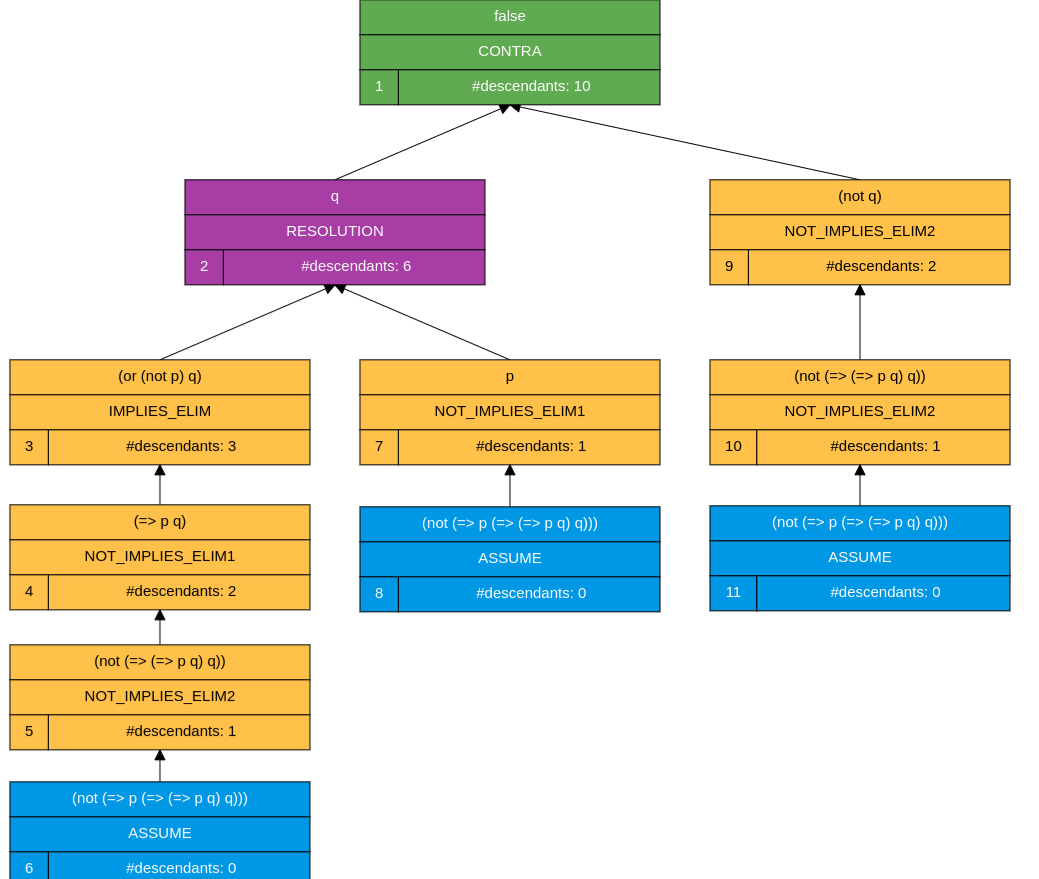
\includegraphics[scale=0.9]{img/mp_cvc5_proof.png}}
  \caption{A cvc5 proof for the validity of Modus Ponens.}
  \label{fig:cvc5-proof}
\end{figure}

The encoding of this proof into Lean requires representing the terms that appear
in it, i.e.\ the formulas built with $p$ and $q$, as well as the rules.
%
This encoding uses a \emph{deep embedding} of the proof calculus of cvc5 into
Lean.
%
It provides a \texttt{term} type that models terms and formulas from MSFOL. This type has
a \texttt{const} constructor for defining symbols, parameterized with an
identifier (a natural number) and a \texttt{sort} (another type for encoding MSFOL
sorts).
%
For example, \texttt{p} and \texttt{q}, which are Boolean constants (MSFOL
constants can be seen as free variables when they are not pre-defined, which is
the case for \texttt{p} and \texttt{q} but not for example for \texttt{false}),
are declared as:

\begin{minted}{lean}
  def p: term := const 1000 boolSort
  def q: term := const 1001 boolSort
\end{minted}

The identifiers \texttt{1000} and \texttt{1001} are arbitrary, with only the
requirement that they are unique.

With these terms and using the functions \texttt{implies} and
\texttt{not} defined in the deep embedding corresponding to the MSFOL symbols
$\rightarrow$ and $\neg$, we encode the formula used in the
query:

\begin{minted}{lean}
  def modusPonensEmbed: term := implies p (implies (implies p q) q)
  def notModusPonensEmbed: term := not modusPonensEmbed
\end{minted}

Finally, the proof from Figure~\ref{fig:cvc5-proof} is encoded as:

\begin{minted}{lean}
  theorem cvc5_th0 : thHolds notModusPonensEmbed -> thHolds bot :=
    fun lean_a0 =>
      have lean_s0 := notImplies2 lean_a0
      have lean_s1 := notImplies1 lean_s0
      have lean_s2 := impliesElim lean_s1
      have lean_s4 := notImplies1 lean_a0
      have lean_s6 := R1 (conjunction lean_s2 lean_s4)
      have lean_s9 := notImplies2 lean_s0
      contradiction (conjunction lean_s9 lean_s6)
\end{minted}
where \texttt{thHolds} is a Lean axiom that lifts a \texttt{term} into a \texttt{Prop}, asserting that it is a valid term.
All the inference rules are encoded as axioms that have the type \texttt{thHolds t1 -> thHolds t2}, for some terms \texttt{t1} and \texttt{t2}. For instance, \texttt{notImplies1} is written in the following form:
\begin{minted}{lean}
  axiom notImplies1 : ∀ {t1 t2 : term},
    thHolds (not (implies t1 t2)) -> thHolds t1
\end{minted}
where the usage of curly brackets indicate that the parameters are implicit.

By applying the rules in the sequence generated by cvc5, we can derive a term
that has type \texttt{thHolds notModusPonens -> thHolds bot}, where \texttt{bot}
is the encoding of MSFOL's $false$.
%
The existence of this term shows that, assuming the rules used by cvc5 are correct, the term \texttt{notModusPonens} is equivalent to \texttt{bot}, which is the same as to say that it is unsatisfiable. This way, we have encoded the proof found by cvc5 inside Lean.

Note that the encoding and printing of the SMT-LIB query as a \texttt{term}, as well as the encoding and printing of the proof, are done automatically by cvc5. On the other hand, the definition of the type \texttt{term} and the declaration of the axioms corresponding to the rules remain static within the module.

    \section{First Approach: Certified Transformations}
    Given this framework for encoding MSFOL in Lean, our goal is to
modify its architecture so that the validity of the rules can be
checked by the kernel, and also, in a way that enables the proofs to refer
to native Lean values, as opposed to only values encoded by the
\texttt{term} type. In this section we describe our first attempt
to achieve this goal, which was using the certified transformations
approach, as described in the introduction.

\subsection{The Boolean Fragment}

Initially, we will limit ourselves to the fragment of MSFOL that
deals with Boolean values\footnote{The Boolean fragment of the
\emph{Core} theory in SMT-Lib, as defined in
\url{http://smtlib.cs.uiowa.edu/theories-Core.shtml}}. Once
we show how to lift this fragment, we will present a generalization
of our definitions that could potentially serve as a basis to lift
any theory from MSFOL.\
%
The first step is to define a function to map values from the \texttt{term} type
to the corresponding native value.

While designing this function, we had a
choice on which type from Lean we would use as a counterpart of \texttt{term}. The two
most suitable alternatives were the \texttt{Prop} and \texttt{Bool} types. The former, as
previously explained, is the type used to model all propositions in the language, while
the latter is the usual type of booleans inhabited by only two values: \texttt{true} and
\texttt{false}. The \texttt{Bool} type has the advantage of potentially not requiring the
\texttt{Classical} module, as it is possible to prove classical statements over them. On
the other hand, propositions in Lean are stated in terms of \texttt{Prop}s.
\tom{I'm not sure about the next statement} Although it is
possible to state them in terms of \texttt{Bool}s, it is not usual. Given that one of the
end goals of our project is to serve as part of a Lean hammer, it is more appropriate
to adopt the most commonly format used. With this in mind, we chose to use \texttt{Prop}.


Note that the term we will evaluate can contain free variables. For those, we will need an auxiliary interpretation function assigning concrete values to them.
Free variables are
identified by a \texttt{Nat} (the built-in Lean type for natural numbers), therefore, we can
represent this information as a function from \texttt{Nat} to
\texttt{Prop}:

\begin{minted}{lean}
  def Interpretation := Nat -> Prop
\end{minted}

With this definition, we can define our evaluation function:

\begin{minted}{lean}
  def evalTerm (I : Interpretation) (t : term) : Prop :=
    match t with
    | term.const   i  _  => I i
    | term.not     t1    => Not (evalTerm I t1)
    | term.and     t1 t2 => And (evalTerm I t1) (evalTerm I t2)
    | term.or      t1 t2 => Or (evalTerm I t1) (evalTerm I t2)
    | term.implies t1 t2 => (evalTerm I t1) -> (evalTerm I t2)
    | term.eq      t1 t2 => (evalTerm I t1) = (evalTerm I t2)
    | term.bot           => False
    | term.top           => True
    | _                  => False
\end{minted}

This function is matching each pattern for a \texttt{term} with the corresponding built-in operation over \texttt{Prop}, and using recursive calls of itself as arguments. If we find a \texttt{term} that is not in the fragment we are currently supporting we just return \texttt{False}. This could potentially lead to consistency issues if the input formula involved other fragments apart from Boolean. As we are limiting ourselves to this fragment, we will ignore this problem for now.

Notice how the \texttt{Interpretation} type we introduced, as well as the evaluation function, match the notions of interpretation and evaluation introduced in Section~\ref{sec:msfolHere}. Indeed, we can now define what it means for an interpretation to satisfy a \texttt{term} and what it means to be unsatisfiable:

\begin{minted}{lean}
  def satisfies (I : Interpretation) (t : term) : Prop :=
    evalTerm I t = True
  def unsatisfiable (t : term) : Prop :=
    ∀ (I : Interpretation), ¬ satisfies I t
\end{minted}

One important concept we need to define is what it means for a \texttt{term}
to follow logically from another, which is the primary relationship modeled
by the axioms presented previously.
%
If, for any fixed interpretation, the evaluation of a given \texttt{term} being true
implies in the evaluation of another \texttt{term} being true, then we can always
conclude the second one from the first. The following definition states this
relationship in Lean:

\begin{minted}{lean}
  def impliesIn (t1 t2 : term) : Prop :=
    ∀ (I : Interpretation),
      satisfies I t1 -> satisfies I t2
\end{minted}

Notice that we needed to use the same interpretation for both terms.
%
The application \texttt{impliesIn t1 t2} gives a precise meaning to \texttt{thHolds t1 -> thHolds t2} in terms of the logic used by Lean.

Since we are interested in proving the unsatisfiability of terms, we will always try to prove a goal of the form \texttt{impliesIn t bot}, for some term \texttt{t}. This would imply that for any interpretation \texttt{I}, we have \texttt{(evalTerm I t = True) -> False}, provided that there is no environment that validates the interpretation of \texttt{bot}. Note that this is equivalent to \texttt{unsatisfiable t}, given our previous definition of \texttt{unsatisfiable}.
With the above we can rephrase and prove the rules from the deep embedding using
\texttt{impliesIn}.
%
For instance, the representation of \texttt{notImplies1} show in Section~\ref{sec:gen-scripts} becomes:

\begin{minted}{lean}
  theorem notImplies1 : ∀ {t1 t2 : term},
      impliesIn (not (implies t1 t2)) t1
\end{minted}

We have proved some of the theorems used in the boolean fragment\footnote{Our proofs can be found at \url{https://github.com/tomaz1502/signatures/blob/smallCheckers/Cdclt/Lift/Other/PropsExample.lean}.}. Their proofs
were straightforward using classical reasoning.

Finally, we can state the theorem from Section~\ref{sec:gen-scripts} as
\texttt{impliesIn notModusPonens bot}, and prove it using almost\footnote{while the original proof used the most general form of resolution, we have restricted ourselves to prove the specific version of resolution that was applied in this proof.} the same
(rephrased) rules in the same order, which already achieves the goal
of checking the proof using Lean's kernel.

In order to apply the generated proof in terms native to the ITP, we need
to prove the following auxiliary theorem:

\begin{minted}{lean}
  theorem notFollowsBot : ∀ {t : term},
    impliesIn (not t) bot → ∀ {I : Interpretation}, evalTerm I t = True
\end{minted}

By applying it on the theorem generated by cvc5, we derive that, for any
interpretation \texttt{I}, \texttt{evalTerm I modusPonensEmbed} is equal
to \texttt{True}:

\begin{minted}{lean}
theorem modusPonensEqTrue: ∀ {I: Interpretation},
    evalTerm I modusPonensEmbed = True :=
  notFollowsBot cvc5_th0
\end{minted}

Now we can define the theorem corresponding to \texttt{cvc5\_th0} using
\texttt{Prop}s and prove it by applying \texttt{modusPonensEqTrue} to
the appropriate interpretation:

\begin{minted}{lean}
def modusPonens (P Q : Prop) : Prop := P → (P → Q) → Q

theorem modusPonensCorrect: ∀ (P Q: Prop), (modusPonens P Q) = True := by
  intros P Q
  exact @modusPonensEqTrue (fun id => if id == 1000 then P else Q)
\end{minted}

where the symbol \texttt{@} is used to make explicit all parameters
in the function after it. Using this interpretation, we indicate
that the term \texttt{p} in \texttt{modusPonensEmbed}
will be matched with the prop \texttt{P} (since the identifier of \texttt{p}
is 1000) and the term \texttt{q} will be matched with the prop \texttt{Q}.
The checker can now compute our evaluation function and
match its return value with \texttt{modusPonens P Q}, thus proving the theorem.

Therefore, we have shown how to lift the proofs produced by cvc5 into proofs
that refer directly to native Lean terms. In order to fully automate this
process, we would have to extend cvc5's module for printing proofs. It would
have to also print, for a given query, the theorem (and its proof, which is always
\texttt{notFollowsBot cvc5\_th0}) corresponding to \texttt{modusPonensEqTrue} for that query,
the representation of the query as a Lean term (which in this example was the term \texttt{modusPonens})
and the theorem that proves that the representation of the query is correct by instantiating the interpretation
properly (corresponding to \texttt{modusPonensCorrect}).
Since we changed our approach, this extension was not realized.

\subsection{Supporting Other Theories}

Supporting more theories from MSFOL requires extending the function \texttt{evalTerm},
as well as the \texttt{Interpretation} type we defined, to be able to return values
of multiple distinct types. One type safe way to achieve this in a language with
dependent types is through a \textit{sigma type}. A sigma type is a pair, in which
the type of the second element depends on the value of the first element. If
\texttt{T} is a type and \texttt{U} is a constructor with type
\texttt{T -> Type}, then \texttt{@Sigma T U} is the type
of pairs \texttt{⟨t, u⟩} such that \texttt{t} has type \texttt{T} and
\texttt{u} has type \texttt{U t}. Note that the first parameter of \texttt{Sigma}
can be inferred from the second, so it is given implicitly.

Let us define a function \texttt{evalSort} that maps the type \texttt{sort}
(corresponding to MSFOL's sorts in the deep embedding) to native Lean types
(which are represented by \texttt{Type}):

\begin{minted}{lean}
  def evalSort : sort -> Type := fun s =>
    match s with
    | arrow s1 s2 => evalSort s1 -> evalSort s2
    | boolSort => Prop
    | intSort => Int
    | _ => Prop
\end{minted}

We have matched the \texttt{arrow} sort with the arrow type used to build the type of
functions, \texttt{boolSort} with \texttt{Prop} and \texttt{intSort} with \texttt{Int}.
For giving support for further theories we have to extend this match statement,
matching the corresponding \texttt{sort} with a suitable type. Since one of the goals
of the project is to be a hammer, it is crucial to choose, for a given sort,
a corresponding type that is most commonly employed by Lean users, and also
has the same properties as the sort.

Now we can reformulate the \texttt{Interpretation} type, in a way that
it supports any type that is also supported by \texttt{evalSort}:

\begin{minted}{lean}
  def Interpretation := Nat → @Sigma sort evalSort
\end{minted}

Given an identifier, an interpretation must return a pair containing its sort
and its value. Note that, with this modification, the interpretation printed
by cvc5 would also need to print the sort of each term. For instance,
the interpretation used in the theorem \texttt{modusPonensCorrect} would have
to be rewritten as:

\begin{minted}{lean}
  def I : Interpretation := fun id =>
    if id == 1000 then
      ⟨ boolSort, P ⟩
    else ⟨ boolSort, Q ⟩
\end{minted}

We will also use a sigma type for defining the new version of \texttt{evalTerm}.
%
Since we are now supporting multiple types, we have to consider what to return
when the input \texttt{term} is ill-typed. One possibility could be to map these
terms to \texttt{False}, as we were doing with \texttt{term}s that were not supported
in the previous version of \texttt{evalTerm}. However, this approach would introduce
a logical inconsistency that would pose challenges to prove some of the rules.
For instance, one rule used by cvc5 is the elimination of double negation:

\begin{minted}{lean}
  theorem notNotElim : ∀ {t : term},
      impliesIn (not (not t)) t
\end{minted}

In order to prove it, we have to consider every possible pattern for \texttt{t}.
If \texttt{t} is not a valid boolean expression, then our evaluation function would
return \texttt{False} for the term \texttt{not t}, which would then force the
evaluation of \texttt{not (not t)} to return \texttt{True}. Since the premiss
is valid in this case, we would have to prove that the conclusion is also valid,
but the conclusion is not a boolean expression. Therefore, the only way to prove it
would be to change our predicate \texttt{satisfies} to accept terms that are not booleans.

Instead of following this approach, we decided to change the evaluation function to just not return
any value if the input term is ill-typed. The polymorphic \texttt{Option} type is used in Lean to
indicate the possible absence of a value, which is represented by \texttt{none}, one of its
constructors. The other constructor, \texttt{some}, receives, as a parameter, a single value
of the type that is used as a parameter to \texttt{Option}.
%
The following snippet shows the reformulated version of \texttt{evalTerm}.
We do not show the complete pattern matching for brevity, but all the other
patterns are implemented using the same structure:

\begin{minted}{lean}
  def evalTerm (I : Interpretation) (t : term) :
      Option (@Sigma sort interpSort) :=
    match t with
    | term.const   i  s  =>
      let ⟨ s', value ⟩ := I i
      if s' == s then some ⟨ s', value ⟩ else none
    | term.and     t1 t2 =>
      match evalTerm I t1, evalTerm I t2 with
      | some ⟨ boolSort, p1 ⟩, some ⟨ boolSort , p2 ⟩ =>
          some ⟨ boolSort, And p1 p2 ⟩
      | _,_ => none
    | _ => none
\end{minted}

We have also reformulated our \texttt{satisfies} predicate, in a way that
it also rejects any term whose evaluation is not a \texttt{Prop}:

\begin{minted}{lean}
  def satisfies (I : Interpretation) (t : term) : Prop :=
    match evalTerm I t with
    | some ⟨ boolSort, p ⟩ => p = True
    | _ => False
\end{minted}

The predicate \texttt{impliesIn} did not require any modification. With these
rephrased definitions we could define and prove new versions of
the theorems regarding the boolean fragment, certifying the validity of the
cvc5 rules over the reformulated version of our framework.

The next step we took was to try to state and prove theorems corresponding to the
axioms from the theory of equality and uninterpreted functions, which
was presented in Section~\ref{sec:euf}. Consider the \texttt{refl} axiom:

\begin{minted}{lean}
  theorem refl : ∀ {I : Interpretation} {t : term}, satisfies I (eq t t)
\end{minted}

If \texttt{t} is ill-typed, then the statement does not hold. This was not
a problem before because all previous axioms were implications in which
the term in the conclusion was a subexpression of the premiss. Therefore,
if the conclusion was ill-typed, the premiss was also, necessarily, ill-typed,
which made the implication true. In the case of \texttt{refl} and of
any other possible theorems that do not have premisses, we have to restrict it
to only refer to well-typed terms in order to make their statement true.

For that purpose, we have defined a new function \texttt{inferSort} that infers the sort of a term
or returns \texttt{none} if it is ill-typed.
This new function is essentially identical to
\texttt{evalTerm}, except that it only computes the first element of the pair.
Also, since the sort of a term is independent of the interpretation we use
to evaluate it, we do not need an interpretation as a parameter in this function.
Now we can make the statement in the theorem \texttt{refl} true by adding the hypothesis
\texttt{isSome (inferSort t) = true}, where \texttt{isSome} is:

\begin{minted}{lean}
  def isSome (opt : Option sort) : Bool :=
    match opt with
    | some _ => true
    | none   => false
\end{minted}

The introduction of this hypothesis creates a new requirement for applying
the theorem in a proof, that is, we have to provide a proof that \texttt{t} is well-typed.
If it is well-typed (which will always be the case as long
as there is no bug in the SMT solver), then Lean's kernel can evaluate
both functions \texttt{inferSort} and \texttt{isSome} and obtain \texttt{true},
and the proof that the term is well-typed follows by reflexivity. Deriving facts
from the evaluation of functions is a proof technique known as \textit{proof by reflection}.
This kind of proof transfer the cost of \textit{checking} the proofs to a cost of
normalizing terms. Unfortunately, as pointed out by~\cite{ringLean}, Lean's evaluator
is not optimized for performance, therefore, the necessity of proving that certain term are
well-typed would probably reduce the efficiency of our tool.

Another downside of this approach is the necessity of providing explicit proofs for the most
general case of all rules. Some of the rules, such as resolution and
\textit{factor} (which takes as premiss a clause and have as a conclusion the same clause, removing
all formulas that are duplicated) appear to lack any proofs that are not highly challenging to derive.
This difficulty is also recognized in~\cite[6]{snipe}:
\begin{quote}
  ``Indeed, the former [certified transformations] require we work only with the reified [meaning deeply embedded] syntax of the
  terms of CIC and even for a simple transformation, the proof of soundess is hard (thousands lines of code).''
\end{quote}

As we will see later, the second approach does not require to build all the proofs \textit{explicitly}.
For those reasons, we decided to change our approach.

% According to~\cite[6]{snipe},

% From leanRingCertifying.pdf (paper about extending ring tactic with certifying
% transformations):
% % \cite{ringLean}
% The ring exp tactic does not use reflection but directly constructs proof
% terms to be type checked by Lean’s kernel, as is typical for tactics in mathlib [10].
% Reflective tactics avoid the construction and checking of a large proof term by
% performing most computation during proof checking, running a verified pro-
% gram [2]. If the proof checker performs efficient reduction, this results in a sig-
% nificant speed-up of the tactic, at the same time as providing more correctness
% guarantees. Unfortunately, the advantages of reflection do not translate directly
% to Lean. Tactic execution in Lean occurs within a fast interpreter, while the
% kernel used in proof checking is designed for simplicity instead of efficient reduc-
% tion [3]. Achieving an acceptable speed for ring exp requires other approaches
% to the benefits that reflection brings automatically.

% \tom{evalterm will have to be evaluated during the checking of the proof produced by cvc5
%   thats a performance issue = references}

% \tom{factor and resolution and permutateOr are exceedingly hard to be proved. From snipe:
% In the work presented in this article, we follow the paradigm of certifying transformations.
% Indeed, the former require we work only with the reified syntax of the terms of CIC and even for
% a simple transformation, the proof of soundess is hard (thousands lines of code).}

% \tom{Haniel said that Chantal said that it is hard to maintain the verification, take a look at her papers}

    \section{Second Approach: Certifying Transformations}
    The second approach, known as certifying
transformations, is based on generating proofs on demand, which will be checked
every time the tool is invoked. The specific manner in which we applied
this concept in our context was to develop a set of tactics matching
each one of the rules present in cvc5's proof calculus.
A cvc5 proof is now represented by a sequence of applications of those tactics.
When we ask Lean's kernel to check a proof, it will execute one by one
of the tactics. Each one of them will inspect the current context
and produce a proof term, corresponding to a proof of a specific
case of the statement represented by that tactic. The checker will then
verify the correctness of each proof, closing the original goal if all
checks were succesful.

The main reason for mapping MSFOL formulas to an inductive type (i.e. \texttt{term})
instead of native Lean expressions was the flexibility achieved by this representation.
While it is straightforward to define a function that inspects and manipulates the
structure of
a \texttt{term} by pattern matching, there is no way to do the same for a \texttt{Prop},
for instance, without recurring to metaprogramming. As we have shown in
Section~\ref{sec:metaLean},
the metaprogramming context grants us access to the internal representation of any
expression
through the \texttt{Expr} type, which can be inspected and manipulated in the same way
as \texttt{term}. Since the framework for writing tactics is based on metaprogramming, we
do not need to rely on the flexibility of the \texttt{term} type anymore. Therefore, we
have decided to not use the deep embedding anymore, and translate MSFOL formulas directly
to Lean expressions.

In the rest of this section we will give an overview of the implementation of each tactic.
We present their statement with the same format used in cvc5's documentation\footnote{The documentation of cvc5's rules can be found at:
  \url{https://cvc5.github.io/docs/cvc5-1.0.2/proofs/proof_rules.html}}, that is,
for a tactic that has a conclusion $\psi$, premisses $\psi_{1} \cdots \psi_{n}$ and
parameters $t_{1} \cdots t_{n}$, we will write:
\[
  \infer[]{\psi}{\psi_{1}, \cdots, \psi_{n} \mid t_{1}, \cdots, t_{n}}
\]

Notice that a large portion of the rules can be trivially proved using classical
reasoning. Instead of mapping those rules to tactics, we just proved them as theorems.
Those theorems will not be presented here. For a complete overview of the rules, their statement and whether they were implemented with a tactic or a
theorem, refer to Table~\ref{tab:rules}.


\subsection*{GroupClausePrefix\\\normalsize{Rule Statement:}}
\[
  \infer[]{(P_{1} \vee \cdots \vee P_{i}) \vee P_{i + 1} \vee \cdots \vee P_{n}}
    {P_{1} \vee \cdots \vee P_{n} \mid i}
\]

\subsection*{LiftOrNToNeg\\\normalsize{Rule Statement:}}
\[
  \infer[]{\neg (P_{1} \wedge \cdots \wedge P_{n})}{(\neg P_{1} \vee \cdots \vee \neg P_{n}) \mid -}
\]


\subsection*{LiftOrNToImp\\\normalsize{Rule Statement:}}
\[
  \infer[]{P_{1} \wedge \cdots \wedge P_{i} \rightarrow P_{i + 1} \vee \cdots \vee P_{n}}{\neg P_{1} \vee \cdots \vee \neg P_{i} \vee P_{i + 1} \vee \cdots P_{n} \mid i}
\]

\subsection*{PermutateClause\\\normalsize{Rule Statement:}}
\[
  \infer[]{P_{p(1)} \vee \cdots \vee P_{p(n)}}{P_{1} \vee \cdots \vee P_{n} \mid p}
\]

\subsection*{Resolution\\\normalsize{Rule Statement:}}
\[
  \infer[]{P_{1} \vee \cdots \vee P_{i - 1} \vee P_{i + 1} \vee \cdots \vee P_{n} \vee Q_{1} \vee \cdots \vee Q_{j - 1} \vee Q_{j + 1} \vee \cdots \vee Q_{m}}{P_{1} \vee \cdots \vee P_{n}, Q_{1} \vee \cdots \vee Q_{m}, P_{i} = Q_{j} \mid i, j}
\]

\subsection*{Factor\\\normalsize{Rule Statement:}}
\[
  \infer[]{removeDuplicates(P_{1} \vee \cdots \vee P_{n})}{P_{1} \vee \cdots \vee P_{n} \mid -}
\]


% \subsection{Pull}

\subsection*{SumBounds\\\normalsize{Rule Statement:}}
\[
  \infer[]{\sum_{i = 1}^{n} a_{i} \bowtie^{*} \sum_{i = 1}^{n} b_{i}}{\bigwedge_{i = 1}^{n} a_{i} \bowtie_{i} b_{i}}
\]

\subsection*{MulPosNeg\\\normalsize{Rule Statement:}}
% \[
%   \infer[]{}{}
% \]


% \subsection{MulPosNeg}

% \subsection{TightBounds}


% TODO: put this in an appendix
\begin{table}[]\label{tab:rules}
\centering
\begin{tabular}{ l l l }
\toprule
Name        & Statement & Implementation \\ \midrule
NotImplies1 & \texttt{Not (p -> q) -> p}      & theorem        \\ \midrule
NotImplies2 & blah      & theorem        \\ \midrule
EquivElim1  & blah      & theorem        \\ \midrule
EquivElim2  & blah      & theorem        \\ \midrule
NotEquivElim1  & blah      & theorem        \\ \midrule
NotEquivElim2  & blah      & theorem        \\ \midrule
ImpliesElim & blah      & theorem        \\ \bottomrule
\end{tabular}
\caption{Rules from cvc5's proof calculus}
\end{table}

	  % \section{Certified vs Certifying}
    %   \label{sec:certifiedVsCertifying}
	  % \section{Classical vs Intuitionist}
	  % \section{Tactics}
	  % \section{The Complete Architecture}
	  % \section{Skipping the Parser}
	  % maybe think of other optimizations and make a section about this
	\chapter{Evaluation}
	\chapter{Future Work}

		%% Referências
		\bibliographystyle{plain}
		\bibliography{referencias}

\end{document}
